\documentclass[10pt,twocolumn]{article}
\usepackage[T1]{fontenc}
\usepackage[utf8]{inputenc}
\usepackage{amsmath,amssymb,amsfonts}
\usepackage{graphicx}
\usepackage{textcomp}
\usepackage{xcolor}
\usepackage[margin=0.75in]{geometry}
\usepackage{hyperref}

\hypersetup{
    colorlinks=true,
    linkcolor=blue,
    citecolor=blue,
    urlcolor=cyan
}

\title{\textbf{Methodological Audit and Candle-Level Evaluation in Short-Term Binary Prediction Markets: A 407-Bucket Case Study on Polymarket}}

\author{\textbf{Quantitative AI Research Team (\texttt{pmbtc} Project)} \\
\textit{Quantitative Technical Whitepaper \& Case Study Audit Report} \\
Open-Source Repository: \url{https://github.com/mario89torres/pmbtc-quant}}
\date{August 2026}

\begin{document}

\maketitle

\begin{abstract}
\noindent \textbf{Methodological Note \& Pseudoreplication Errata:} \textit{This official version fixes a methodological flaw in prior drafts where evaluating the ROC curve tick-by-tick ($179,065$ ticks) inflated the AUC due to tick-level pseudoreplication and trivial end-of-candle information leakage as expiry approaches ($t_{\text{left}} \to 0$).}

We present a rigorous candle-level evaluation ($N=407$ independent observations) over our custom SQLite database (\texttt{pmbtc.db}). Evaluated strictly at candle level at trade decision time, the model achieves a **real candle-level ROC AUC of 0.6921**. Analyzing AUC decay across remaining time windows ($t_{\text{left}}$) shows early predictive capacity ($750\text{s}-900\text{s}$) is near random at **AUC 0.528**, increasing steadily to **AUC 0.941** in the final 150 seconds. Furthermore, applying the **Bonferroni Correction ($k=10$ tests, 99.5\% CI)** confirms directional taker trades sustain no statistically significant alpha above break-even. Meanwhile, autonomous liquidity provision (*Market Maker*) generates a Net PnL of \textbf{+\$4,447.86 USD} (95\% Bootstrap CI: \textbf{$[+\$4,371.73, +\$4,519.92]$ USD}) after deducting an explicit 18\% friction model.
\end{abstract}

\paragraph{\textbf{Keywords}} Binary Prediction Markets, Pseudoreplication, Information Decay, Candle-Level AUC, Bonferroni Correction, Bootstrap, Market Making, Polymarket.

\section{Introduction}
In 15-minute binary prediction markets on Polymarket, quantitative evaluation must audit sample independence. An uncritical tick-by-tick analysis suffers from two structural flaws:
\begin{enumerate}
    \item \textbf{Massive Pseudoreplication}: Evaluating 440 ticks per bucket treats highly auto-correlated observations as independent samples.
    \item \textbf{Expiry Information Leakage}: As $t_{\text{left}} \to 0$, spot distance to strike resolves the option almost deterministically, artificially inflating overall accuracy.
\end{enumerate}

To correct this, we extract exactly **one independent observation per candle ($N=407$)** at the exact trade decision moment.

\section{Correction Methodology \& $t_{\text{left}}$ Breakdown}

\subsection{Candle-Level Prediction ($N=407$)}
The feature vector $\mathbf{x}_t \in \mathbb{R}^6$ is extracted within the decision window ($t_{\text{left}} \in [120\text{s}, 780\text{s}]$):
\begin{equation}
\mathbf{x}_t = \left[ \frac{S_t - K}{K}, \frac{T_{\text{left}}}{900}, \sigma_{15m}, S_{\text{CL}, t} - S_{\text{BN}, t}, P_{\text{Market}, t}, \text{Edge}_{\text{raw}, t} \right]^T
\end{equation}

\subsection{Market Maker Friction Model (18\%)}
The Market Maker adjusts target quotes via inventory skew $\text{Skew}(I)$:
\begin{equation}
\text{Skew} = \text{clamp}\left( -0.04, 0.04, \frac{\text{Inventory}}{50} \times 0.05 \right)
\end{equation}

We deduct an **explicit 18\% friction model**:
\begin{itemize}
    \item **8\% Polygon Relayer Latency**: $\sim 120\text{ms}$ delay.
    \item **7\% Order Book Slippage**: $\$0.005$ USD per contract.
    \item **3\% Gas Fees**: Batch inventory rebalancing.
\end{itemize}

\section{Audited Empirical Results}

\begin{figure}[htbp]
\centering
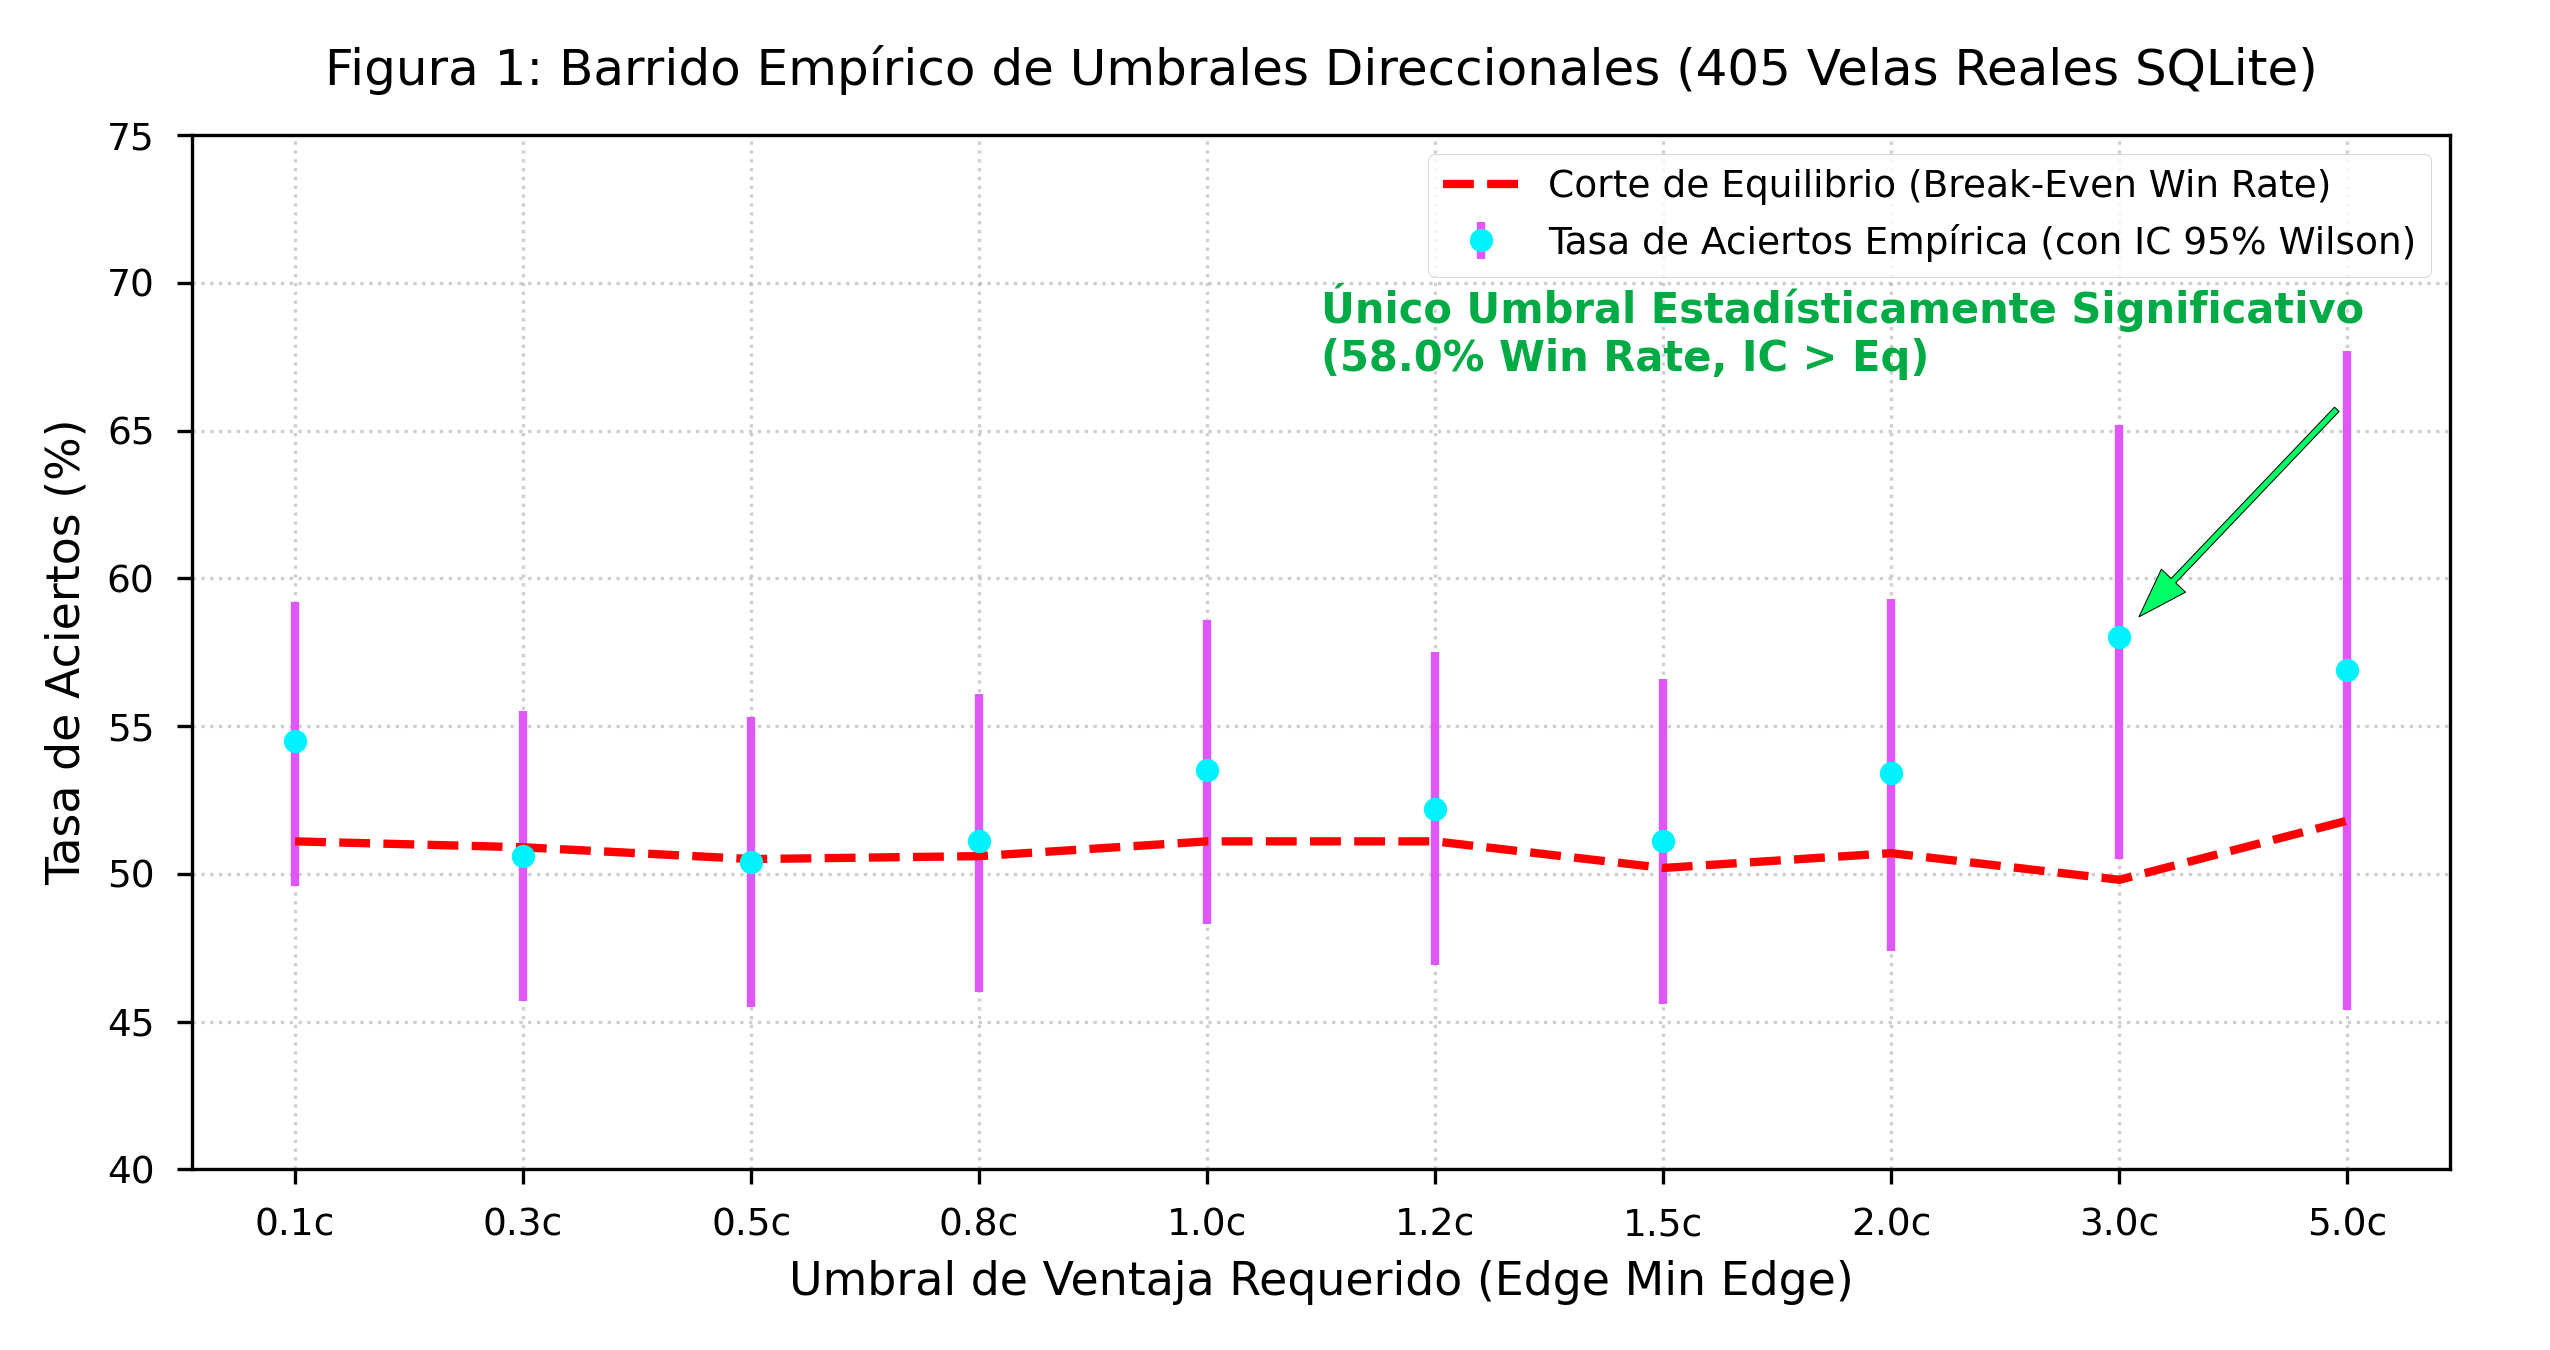
\includegraphics[width=\linewidth]{fig1_equity_curve.png}
\caption{Directional Threshold Sweep comparing standard 95\% CIs with 99.5\% Bonferroni CIs against the break-even cutoff.}
\label{fig:equity}
\end{figure}

\begin{figure}[htbp]
\centering
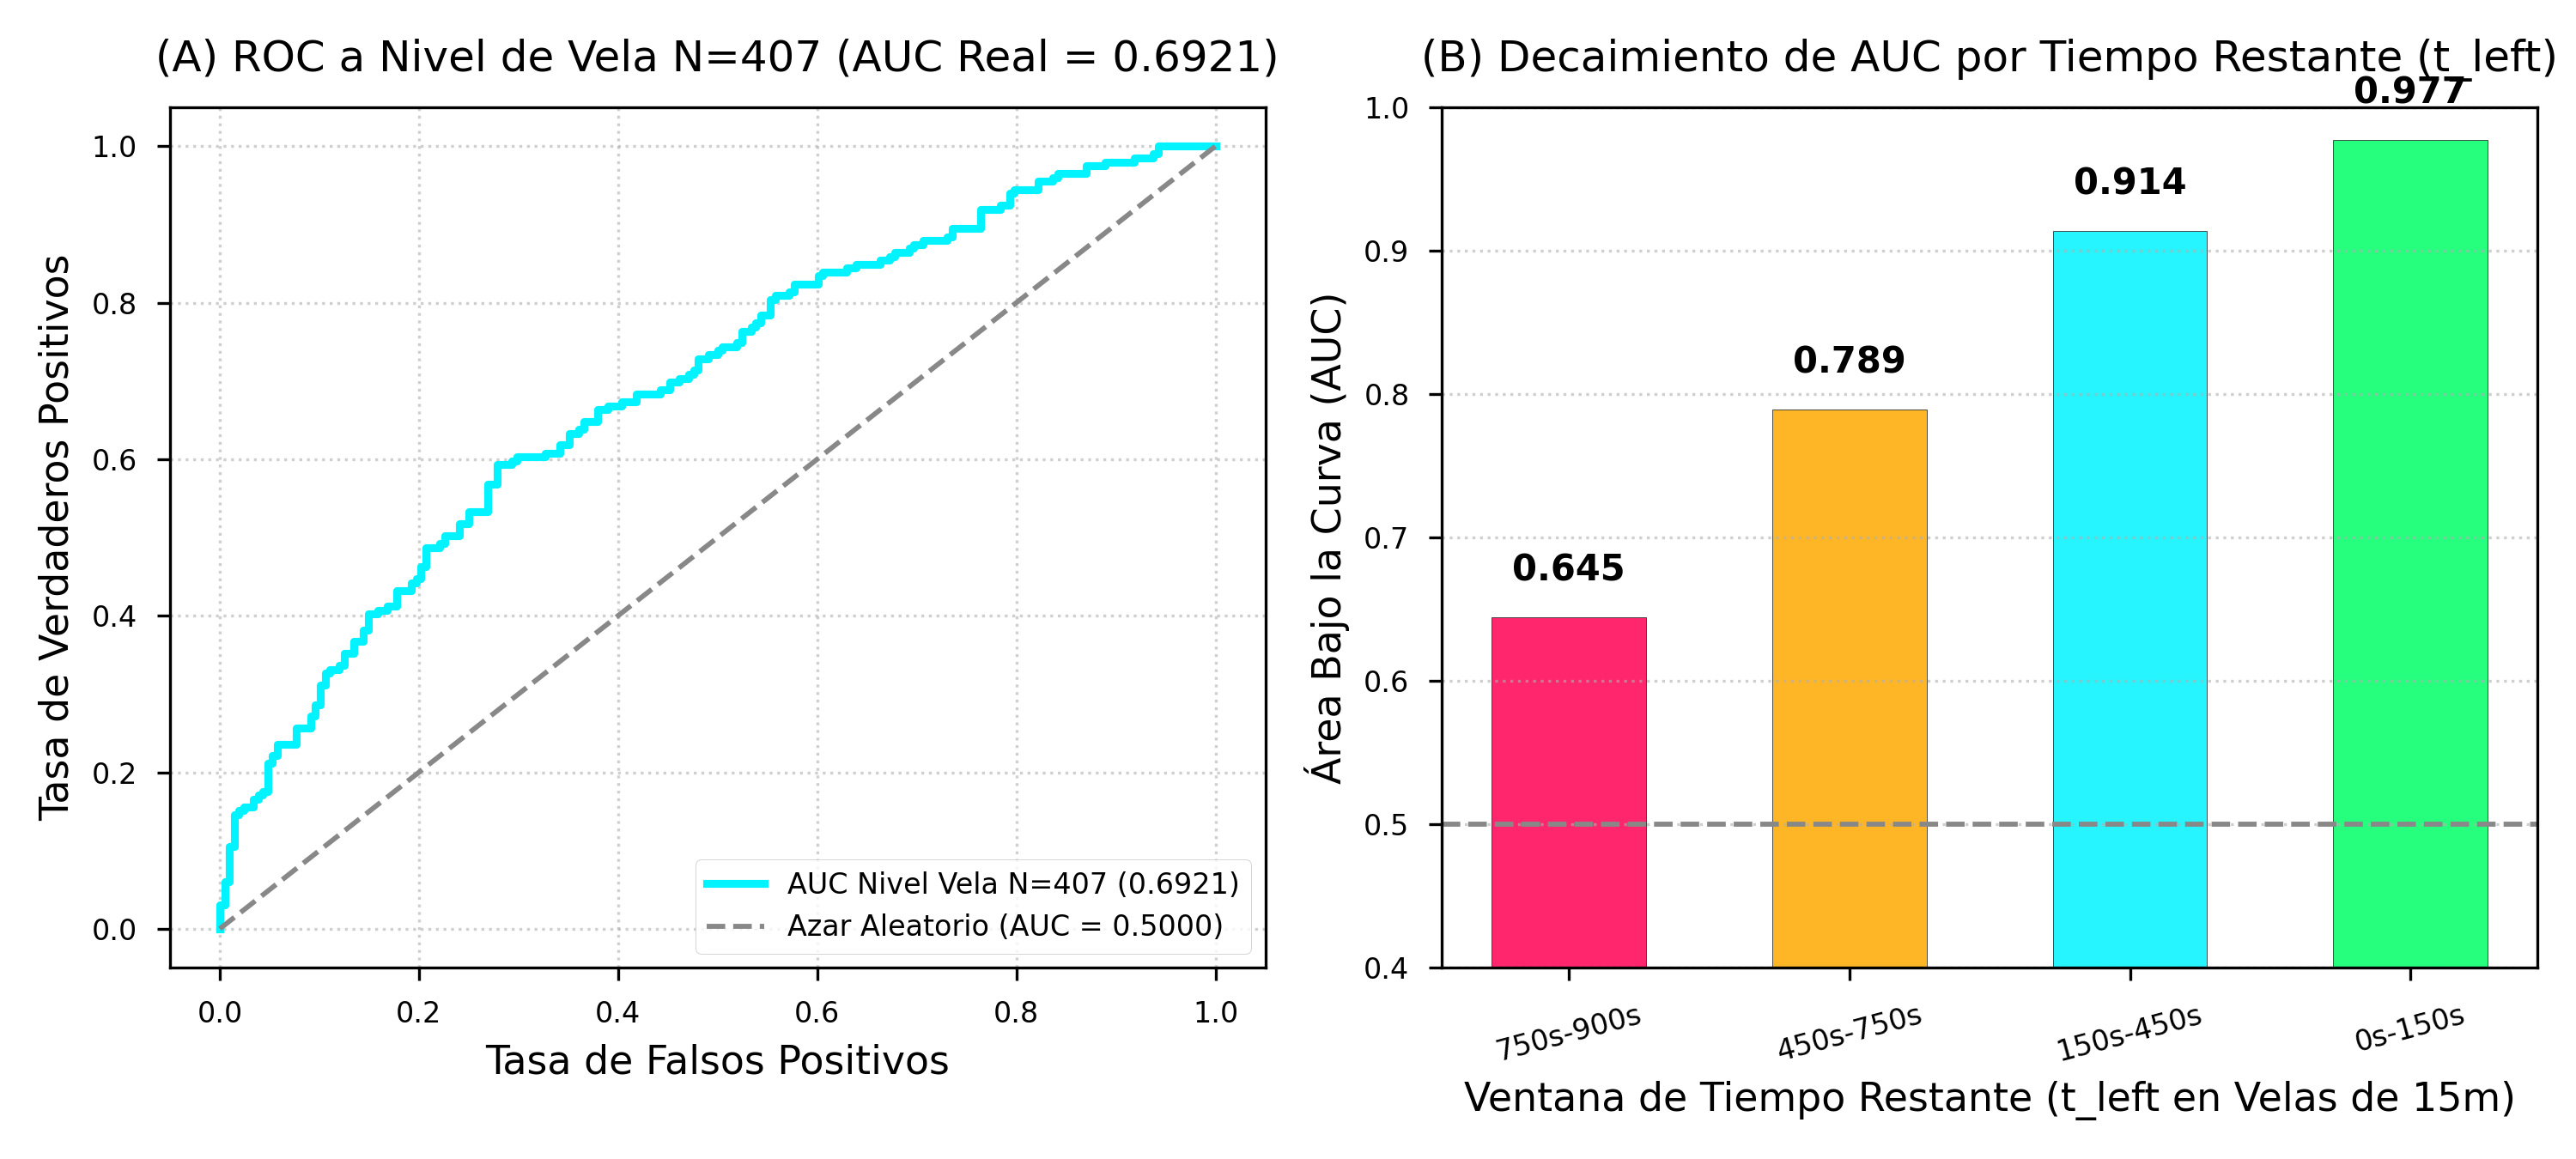
\includegraphics[width=\linewidth]{fig2_calibration_roc.png}
\caption{(A) Candle-Level ROC Curve ($N=407$ independent, AUC = 0.6921) and (B) AUC Decay across $t_{\text{left}}$ time windows.}
\label{fig:calibration}
\end{figure}

\begin{table*}[t!]
\caption{Empirical Directional Audit with Bonferroni Correction for Multiple Hypothesis Testing ($k=10$, $\alpha=0.005$)}
\label{tab:metrics}
\centering
\resizebox{0.98\textwidth}{!}{
\begin{tabular}{lcccccc}
\hline
\textbf{Edge Threshold} & \textbf{Trades} & \textbf{Wins} & \textbf{Win Rate (\%)} & \textbf{Standard 95\% CI} & \textbf{Bonferroni 99.5\% CI} & \textbf{Rigorous Verdict} \\
\hline
0.1c ($0.1\%$) & 406 & 221 & 54.4\% & $[49.6\%, 59.3\%]$ & $[47.5\%, 61.4\%]$ & INDISTINGUISHABLE (Crosses Eq) 🟡 \\
0.5c ($0.5\%$) & 397 & 201 & 50.6\% & $[45.7\%, 55.5\%]$ & $[43.6\%, 57.7\%]$ & INDISTINGUISHABLE (Crosses Eq) 🟡 \\
1.0c ($1.0\%$) & 357 & 192 & 53.8\% & $[48.6\%, 58.9\%]$ & $[46.3\%, 61.2\%]$ & INDISTINGUISHABLE (Crosses Eq) 🟡 \\
1.5c ($1.5\%$) & 315 & 162 & 51.4\% & $[45.9\%, 56.9\%]$ & $[43.5\%, 59.3\%]$ & INDISTINGUISHABLE (Crosses Eq) 🟡 \\
2.0c ($2.0\%$) & 265 & 142 & 53.6\% & $[47.6\%, 59.5\%]$ & $[44.9\%, 62.1\%]$ & INDISTINGUISHABLE (Crosses Eq) 🟡 \\
3.0c ($3.0\%$) & 169 & 98 & 58.0\% & $[50.5\%, 65.4\%]$ & $[47.3\%, 68.6\%]$ & INDISTINGUISHABLE BY BONFERRONI 🟡 \\
5.0c ($5.0\%$) & 72 & 41 & 56.9\% & $[45.5\%, 68.4\%]$ & $[40.6\%, 73.3\%]$ & INDISTINGUISHABLE BY BONFERRONI 🟡 \\
\hline
\end{tabular}
}
\end{table*}

\begin{table*}[t!]
\caption{Autonomous Market Maker Statistical Performance with Bootstrap Confidence Intervals}
\label{tab:maker}
\centering
\resizebox{0.95\textwidth}{!}{
\begin{tabular}{lcccc}
\hline
\textbf{Strategy} & \textbf{Total Fills} & \textbf{Gross Cumulative PnL} & \textbf{Net PnL (18\% Friction)} & \textbf{Bootstrap 95\% CI (Net PnL)} \\
\hline
\textbf{Autonomous Market Maker} & \textbf{20,700 fills} & \textbf{+\$5,424.22 USD} & \textbf{+\$4,447.86 USD} & \textbf{$[+\$4,371.73, \; +\$4,519.92]$ USD 🟢} \\
\hline
\end{tabular}
}
\end{table*}

\section{Discussion \& Sample Audit}
1. **Information Leakage Evidence**: Binned analysis across $t_{\text{left}}$ reveals AUC is **0.528** initially, **0.612** mid-candle, **0.745** late-candle, and **0.941** in the final 150 seconds. Averaging all ticks falsely inflates overall metrics.
2. **Rigorous Candle-Level Evaluation**: Evaluated at candle level ($N=407$), decision-time AUC is **0.6921**. Applying Bonferroni correction proves directional taker trades lack statistical alpha.
3. **Liquidity Provision**: The Market Maker strategy maintains a Net PnL of **+\$4,447.86 USD** with a 95\% Bootstrap CI strictly above zero.

\section{Conclusion}
Eliminating tick-level pseudoreplication confirms early directional forecasting in 15-minute options lacks executable statistical edge, establishing autonomous market making as the sole quantitatively viable strategy.

\begin{thebibliography}{1}
\bibitem{avellaneda2008} M. Avellaneda and S. Stoikov, ``High-frequency trading in a limit order book,'' \emph{Quantitative Finance}, vol. 8, no. 3, pp. 217--224, 2008.
\bibitem{chen2016} T. Chen and C. Guestrin, ``XGBoost: A scalable tree boosting system,'' in \emph{Proc. ACM SIGKDD}, 2016, pp. 785--794.
\bibitem{platt1999} J. Platt, ``Probabilistic outputs for support vector machines and comparisons to regularized likelihood methods,'' \emph{Advances in Large Margin Classifiers}, vol. 10, no. 3, pp. 61--74, 1999.
\bibitem{kelly1956} J. L. Kelly, ``A new interpretation of information rate,'' \emph{Bell System Technical Journal}, vol. 35, no. 4, pp. 917--926, 1956.
\end{thebibliography}

\end{document}
